%!TEX root = ../main.tex

\section*{Ejercicio 5}
Considere el sistema $Ax = b$ donde
\[
A = \begin{bmatrix} 3 & -1 & -1 & 0 & 0 \\ -1 & 4 & 0 & -2 & 0 \\ -1 & 0 & 3 & -1 & 0 \\ 0 & -2 & -1 & 5 & -1 \\ 0 & 0 & 0 & -1 & 2 \end{bmatrix}, \quad b = \begin{bmatrix} 2 \\ -26 \\ 3 \\ 47 \\ -10 \end{bmatrix}
\]
\begin{enumerate}
    \item[a)] Investigue la convergencia de los métodos de Jacobi, Gauss-Seidel y sobrerelajación.

    \begin{solution}
    Para determinar la convergencia del método de Jacobi basta observar que la matriz A es estrictamente diagonal-dominante por filas, por lo tanto el método de Jacobi converge. Al programar el método y con una tolerancia de 0.001 respecto al error en \\ $\|\cdot\|_{\infty}$ se observa que el método se detiene luego de 28 iteraciones y se obtiene un error de aproximadamente $7.7359\times10^{-4}$.

    Veamos ahora que A es simétrica definida positiva, pues así garantizamos la convergencia del método de sobrerelajación para $\omega \in (0,2)$ y por lo tanto del método de Gauss - Seidel. Procederemos a calcular $x^TAx$ para un vector no nulo arbitrario:

    \begin{align*}
        x^TAx&=\begin{bmatrix}
            x_1 & x_2 & x_3 & x_4 & x_5 
        \end{bmatrix} \begin{bmatrix}
            3 & -1 & -1 & 0 & 0 \\
            -1 & 4 & 0 & -2 & 0 \\ 
            -1 & 0 & 3 & -1 & 0 \\
            0 & -2 & -1 & 5 & -1 \\
            0 & 0 & 0 & -1 & 2
        \end{bmatrix}\begin{bmatrix}
            x_1\\
            x_2\\ 
            x_3\\
            x_4\\ 
            x_5\\ 
            \end{bmatrix}\\
            &= \begin{bmatrix}
            x_1 & x_2 & x_3 & x_4 & x_5
            \end{bmatrix} \begin{bmatrix}
            3x_1 - x_2 - x_3 \\ 
            -x_1 + 4x_2 -2x_4 \\ 
            -x_1 +3x_3 -x_4 \\ 
            -2x_2 - x_3  + 5x_4 - x_5 \\ 
            -x_4 + 2x_5\\ 
            \end{bmatrix}\\ 
            &= 3x_1^2 + 4x_2^2 + 3x_3^2 + 5x_4^2 + 2x_5^2 -2x_1x_2 -2x_1x_3 - 4x_2x_4 -2x_3x_4 - 2x_4x_5\\
            &= (x_1 - x_2)^2 + (x_1 - x_3)^2 + 2(x_2 - x_4)^2 + (x_3 - x_4)^2 + (x_4 - x_5)^2 + x_1^2 + x_2^2 + x_3^2 + x_4^2 + x_5^2 \\ 
            & > 0
    \end{align*}
    Con esto vemos que $x^TAx > 0$ y por lo tanto $A$ es definida positiva, así, los métodos de sobrerelajación con $\omega \in (0,2)$ y de Gauss-Seidel convergen. 
    Al programar el método de Gauss-Seidel y fijar la misma tolerancia que con el método de Jacobi, éste se detiene luego de 14 iteraciones y un error de aproximadamente $6.8814 \times 10^{-4}$, con lo cual notamos que el método converge significativamente más rápido que el de Jacobi. 
    Ahora, si programamos el método de sobrerelajación tomando $\omega = 1.18$ usando las mismas condiciones de parada anteriores, éste se detiene luego de 9 iteraciones, por tanto podemos decir que de los tres métodos, es el que converge más rápido. 
    \end{solution}

    \item[b)] ¿Cuál es el radio espectral de la matriz $J$ y de la matriz $S$?

    \begin{solution}
        Para esto primero calculamos las matrices $T_J$ y $T_{GS}$ en Matlab de acuerdo a las fórmulas $T_J=D^{-1}(U+L)$ y $T_{GS} = (D-L)^{-1}U$ y luego calculamos el radio espectral usando el siguiente código
        \begin{lstlisting}
    T_J=inv(D)*(L+U); 
    T_GS=inv(D-L)*U;
    p_J=max(abs(eig(T_J))); %radio espectral de T_J
    p_GS = max(abs(eig(T_GS))); %radio espectral de T_GS
        \end{lstlisting}
        así obtuvimos que $\rho(T_J) = 0.7158$ y $\rho(T_{GS}) = 0.5123$, observe que $\rho(T_J) < \rho(T_{GS})$, lo cual es esperable pues el radio espectral determina la velocidad de convergencia de cada método.
    \end{solution}

    \item[c)] Aproxime con dos cifras decimales el parámetro de sobrerelajación $\omega^*$.

    \begin{solution}
        Teniendo en cuenta que el radio espectral determina la velocidad de convergencia, podemos calcular el radio espectral de la matriz de iteración, variando $\omega$ entre 0 y 2, con pasos de $0.01$ para obtener la precisión deseada, luego escogemos el $\omega$ que minimice el radio espectral de la matriz $T_\omega$. En este caso obtuvimos que el parámetro $\omega^*$ es aproximadamente 1.18, como se observa en la gráfica:
        \begin{center}
    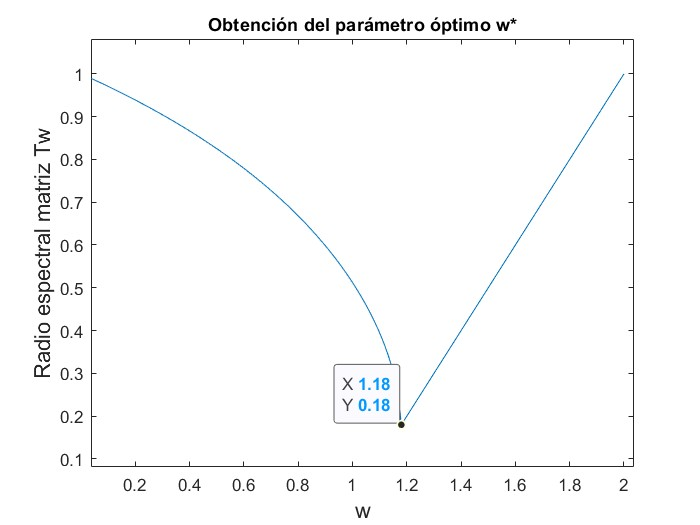
\includegraphics[scale=0.5]{Graficas/Punto5c.jpg}
        \end{center}
    \end{solution}
    \item[d)] ¿Qué reducción en el costo operacional ofrece el método de sobrerelajación con el parámetro $\omega^*$, en comparación con el método de Gauss-Seidel?
    \begin{solution}
        La reducción en el costo operacional puede interpretarse como la diferencia en el número de iteraciones de cada método, pues en general cada iteración tiene el mismo número de operaciones, sin tener en cuenta el cálculo de las matrices de iteración, pues éste se puede realizar antes de implementar cada método. En ese caso, programamos ambos métodos variando la tolerancia al error, de tal manera que se pudiera evidenciar la diferencia entre las iteraciones de cada método.
        De esta forma obtenemos la siguiente tabla:
\begin{center}
\begin{tabular}{|l|l|l|l|l|l|l|l|l|l|l|l|l|l|c|}\hline
Tolerancia & 1 & $10^{-1}$ & $10^{-2}$ & $10^{-3}$ & $10^{-4}$ & $10^{-5}$ & $10^{-6}$ & $10^{-7}$ & $10^{-8}$ & $10^{-9}$ & $10^{-10}$ \\ \hline
Sobrerelajación & 4 & 6 & 7 & 9 & 10 & 11 & 12 & 14 & 15 & 16 & 17 \\ \hline
Gauss-Seidel & 4 & 8 & 11 & 15 & 18 & 22 & 25 & 28 & 32 & 35 & 39 \\ \hline      
\end{tabular}
\end{center}
Aquí observamos que a medida que la tolerancia se hace más pequeña, la relación entre la cantidad de iteraciones de cada método es aproximadamente 0.43, lo cual significa que con el metodo de Sobrerelajación reducimos la cantidad de operaciones en un $56\%$ con respecto al método de Gauss-Seidel.
    \end{solution}
    \item[e)] ¿Cuántas iteraciones más requiere el método de Gauss-Seidel para lograr una precisión mejorada en una cifra decimal? ¿Cuántas necesita el método de sobrerelajación con $\omega^*$?
    \begin{solution}
        Si observamos nuevamente la tabla del inciso anterior, variamos la tolerancia justamente para que cada vez se mejore la precisión en una cifra decimal, y notamos que para el método de Gauss-Seidel se necesitan al rededor de 3 o 4 iteraciones más para lograr esto. En cambio, para lograr esta misma mejoría en la precisión con el método de sobrerrelajación, basta iterar 1 o 2 veces más, lo cual también indica que éste método converge mucho más rápido que el anterior.
    \end{solution}
\end{enumerate}
